% Build with `tectonic -X compile bimetal.tex` in this folder.
\documentclass[sigconf,nonacm]{acmart}
\settopmatter{printacmref=false,printfolios=true,printccs=false}
\renewcommand\footnotetextcopyrightpermission[1]{}
\pagestyle{plain}
\citestyle{acmnumeric}
% The look of every diagram, defined once.
\usepackage{tikz}
\usetikzlibrary{arrows.meta,positioning,fit,calc,backgrounds,decorations.pathreplacing,patterns}

% Okabe and Ito's palette, which survives colour blindness, with gray for everything unemphasised.
\definecolor{ink}{HTML}{1F2933}
\definecolor{quiet}{HTML}{6B7280}
\definecolor{rule}{HTML}{D5D9DE}
\definecolor{python}{HTML}{0072B2}
\definecolor{wasm}{HTML}{D55E00}
\definecolor{addon}{HTML}{009E73}
\definecolor{amber}{HTML}{E69F00}
\definecolor{plum}{HTML}{CC79A7}

\tikzset{
  >={Stealth[length=4.2pt,width=3.4pt]},
  every picture/.append style={line width=0.55pt, font=\footnotesize, text=ink},
  part/.style={draw=python, fill=python!9, rounded corners=1.8pt, align=center,
    minimum height=6.6mm, inner xsep=3pt, inner ysep=1.5pt, font=\scriptsize},
  object/.style={draw=quiet, fill=rule!45, rounded corners=1.8pt, align=center,
    minimum height=7mm, inner xsep=3pt, inner ysep=1.5pt, font=\scriptsize},
  yours/.style={draw=ink, fill=white, rounded corners=1.8pt, align=center,
    minimum height=7mm, inner xsep=3pt, inner ysep=1.5pt, font=\scriptsize},
  boundary/.style={draw=quiet, dashed, rounded corners=4pt},
  flow/.style={->, draw=python, line width=0.7pt},
  plain/.style={->, draw=quiet, line width=0.55pt},
  note/.style={font=\scriptsize, text=quiet, align=center, inner sep=1pt},
  tag/.style={font=\scriptsize, fill=white, inner sep=1pt, align=center},
  stepmark/.style={circle, draw=ink, fill=white, font=\tiny\bfseries, inner sep=0.6pt, minimum size=3.2mm},
}

\newtheorem{claim}{Claim}
\newcommand{\ttt}[1]{\texttt{#1}}
\emergencystretch=1.5em


\begin{document}

\title{Bimetal: One Rust API for Python, Node.js and the Browser}
\author{Felipe Faria}

\begin{abstract}
Bimetal turns one Rust library into a Python package and a TypeScript package that call the same compiled code. Today, an author who wants both packages writes a binding layer for each language, and then keeps the types, the validation and the documentation of the two layers in agreement by hand. Bimetal instead reads the API from the compiled library: marked Rust items register a description of themselves when they are compiled, and a command loads a build of the library and asks it for that description. From the description, generators write Pydantic models, TypeScript declarations and a class for each Rust value that stays alive between calls. The generated files are committed, and a check fails when a fresh build produces different bytes. Because Python, WebAssembly and Node.js differ in what a call may do, this paper also states what each one promises when another call is using a value, when a call is cancelled and when Rust panics. On a laptop, a call with no arguments takes 53~ns in Python, and a batch of a million Arrow rows passes from Python into Rust and back in 4.8~$\mu$s.
\end{abstract}

\keywords{language bindings, foreign function interfaces, code generation, WebAssembly, reproducible builds}

\maketitle

\section{Introduction}

A useful library written in Rust eventually needs callers that do not write Rust. The usual answer is a binding layer for each language: PyO3~\cite{pyo3} for Python, napi-rs~\cite{napirs} for Node.js and wasm-bindgen~\cite{wasmbindgen} for the browser. Each of these tools does its job well, but each asks the author to describe the API again for that language alone. The Python types then need stubs, which PyO3's guide suggests maintaining by hand~\cite{pyo3typing}, the data types need validation in each language, and the documentation needs copying. The author ends up with three descriptions of one API and nothing that keeps them in agreement.

Generating bindings from one definition is an old idea, from SWIG~\cite{beazley1996swig} and Thrift~\cite{slee2007thrift} to UniFFI~\cite{uniffi} and Diplomat~\cite{diplomat}. Doing it for Python and the browser together is hard for two reasons. The first is that the runtimes differ in what a call may do. A Python call can block its thread on a lock, whereas JavaScript has a single thread that cannot wait for itself. Python can share Arrow memory with Rust, but JavaScript cannot, because a view into WebAssembly memory is detached whenever that memory grows. A native library can catch a panic, while in WebAssembly a panic is a trap that leaves the module's memory in an unknown state~\cite{haas2017wasm}. The second reason is that generated code is useful only while it matches the Rust code. A separate interface file can drift from the Rust code, and so can a parser that reads Rust source, because a \ttt{cfg} attribute, a macro or a build script can change what the compiler builds.

Existing tools avoid these problems by narrowing their scope. PyO3, napi-rs and wasm-bindgen give full control of one runtime, and the author repeats the work for the next one. UniFFI and Diplomat generate bindings for many languages, but in each language they support fewer types and language features than the single-language tools do.

Bimetal starts from one observation: a compiled library already contains an exact description of what the compiler built. Each marked item registers a description of itself when it is compiled. To read the API, a command builds the library for the current machine, loads the build, and calls a function that returns a JSON description, which we call the \emph{contract}. Generators write a package for each language from the contract, and the author commits these packages to the repository. A change to the API therefore appears in code review, and a later build can compare the committed files with what the Rust code would generate.

This design makes three trade-offs. First, Bimetal generates code for two languages only, because each language needs its own generator, its own runtime and its own implementation of every feature. Second, a call passes through generated code that validates and converts its values, which costs time that a hand-written binding does not spend (Section~\ref{sec:costs}). Third, where the runtimes differ, the packages differ too: a panic ends a WebAssembly module, and a synchronous method on a value that another call is using throws in JavaScript where it would wait in Python.

This paper makes the following contributions:
\begin{itemize}
  \item A way to read an API from compiled Rust through a small C interface, and a set of checks that each compiled artifact agrees with what was read (Section~\ref{sec:contract}).
  \item One function that plans the native code for three runtimes, which decodes each value once, and a count of the copies each runtime makes (Sections~\ref{sec:wrappers} and~\ref{sec:values}).
  \item A design for stateful values that keeps Rust's aliasing rule across the language boundary, with a statement of what each runtime does when another call is using a value (Section~\ref{sec:resources}).
  \item A guard that makes every pending and later call fail with an error after a WebAssembly trap, where the trap alone would leave promises pending for ever (Section~\ref{sec:failures}).
  \item The rules that make a committed WebAssembly module reproducible across checkouts, and a division of a build's inputs that keeps a committed fingerprint equal on every machine (Section~\ref{sec:reproducible}).
\end{itemize}

\section{Background and Model}
\label{sec:model}

\subsection{What the Hosts Offer}

Bimetal runs Rust code inside another language's runtime in three ways, each of which we call a \emph{host}. The \emph{extension} is a CPython extension built on PyO3, and it serves Python. The \emph{module} is a WebAssembly module built on wasm-bindgen, and it serves TypeScript in Node.js and in browsers. The \emph{addon} is a Node.js addon built on Node-API~\cite{nodeapi}, and it serves TypeScript in Node.js alone. We refer to the extension and the addon together as the \emph{native hosts}, and to the module and the addon as the \emph{JavaScript hosts}. An application enables the extension, one of the JavaScript hosts, or both.

Table~\ref{tab:hosts} compares the three hosts, and two of its rows shape most of the design. A host that cannot block a thread cannot make a synchronous call wait for a lock, and a host that cannot share memory with Rust must copy every large value.

\begin{table}[t]
\caption{The three hosts, and what each one offers.}
\label{tab:hosts}
\small
\begin{tabular}{@{}p{0.34\linewidth}p{0.18\linewidth}p{0.18\linewidth}p{0.17\linewidth}@{}}
\toprule
 & Extension & Module & Addon \\
\midrule
Compiled file & \ttt{.abi3.so} & \ttt{.wasm} & \ttt{.node} \\
One build serves & A platform & All platforms & A platform \\
Runs in browsers & No & Yes & No \\
Threads in Rust & Yes & No & Yes \\
Async calls that wait run on & Tokio & Event loop & Tokio \\
A sync call can wait & Yes & No & No \\
Shares Arrow memory & Yes & No & No \\
Usable after a panic & Yes & No & Yes \\
\bottomrule
\end{tabular}
\end{table}

\subsection{Assumptions}

An \emph{application} is one Cargo package with a file called \ttt{bimetal.toml} beside it. The promises that this paper makes about an application depend on five assumptions.

\begin{description}
\item[A1, build inputs.] Cargo's dependency files list every file that a build reads, and they name every environment variable that a build reads.
\item[A2, a deterministic compiler.] The same toolchain, sources and flags produce the same bytes.
\item[A3, one API on every target.] An exported item has the same signature and the same types on every compilation target.
\item[A4, runtimes as documented.] CPython continues to honour its stable interface~\cite{pep384}, Node.js continues to honour Node-API, and growing a WebAssembly memory detaches its views.
\item[A5, one trust domain.] The caller and the Rust code form one program. Validation catches mistakes, and it does not defend against a hostile caller.
\end{description}

The first three assumptions can fail in practice, and each failure has a remedy. A1 fails when a build script or a procedural macro reads an input without telling Cargo, in which case a build can report that nothing changed when something did, and \ttt{bimetal build --force} recovers. A2 is at risk because local paths are among a build's inputs and differ between machines. Section~\ref{sec:reproducible} describes how the command removes them, and if A2 still fails, \ttt{bimetal check --rebuild} reports the difference. An author can break A3 with a \ttt{cfg\_attr} that renames a field on one target, and a call on that target can then fail when it decodes a value. Section~\ref{sec:contract} describes what the command checks in place of A3.

\subsection{Goals and Non-Goals}

The design has four goals, in priority order: generated code that cannot silently differ from the Rust code, an API that follows each language's conventions, failures that say what happened, and calls that pay only for the checks they need.

Four things are outside the design. Bimetal does not support other languages. An author cannot shape a class differently in each language, because one signature has to mean the same thing everywhere. A call is not as cheap as a hand-written one. Finally, Rust is not isolated from its caller, so a stack overflow in Rust ends the process on a native host.

\section{Overview}
\label{sec:overview}

An author marks the items of a Rust library that callers may use. We say that a value \emph{crosses} when it moves between Rust and Python or JavaScript, and we call the point where this happens the \emph{boundary}. Two kinds of item cross. A \emph{model} is a type that crosses as data, and it derives \ttt{Model} together with Serde's \ttt{Serialize} and \ttt{Deserialize}. A \emph{resource} is a Rust value that stays alive between calls, and its \ttt{impl} block takes the attribute \ttt{\#[bimetal::export]}, as does a free function. The rest of this paper uses one running example, a small library called \ttt{greeter}:

\begin{footnotesize}
\begin{verbatim}
#[derive(Serialize, Deserialize, Model)]
pub struct GreetingRequest {
    #[bimetal(min_length = 1, max_length = 64)]
    pub name: String,
    pub tone: Tone,
}

#[bimetal::export]
pub fn greet(request: GreetingRequest)
    -> Result<Greeting, GreeterError> { ... }

#[bimetal::export]
impl Guestbook {
    #[bimetal(constructor)]
    pub fn new(event: String) -> Self { ... }
    pub fn sign(&mut self, name: String)
        -> Result<(), GreeterError> { ... }
}
\end{verbatim}
\end{footnotesize}

\begin{sloppypar}
The attribute \ttt{min\_length} is a \emph{field rule}: a limit on a model's field that every host enforces. A Python caller writes \ttt{greet(GreetingRequest(\allowbreak name="Ada",\allowbreak{} tone=Tone.Formal))} and receives an immutable Pydantic model~\cite{pydantic}, while a TypeScript caller writes \ttt{greet(\{name: "Ada",\allowbreak{} tone: Tone.Formal\})} and receives a frozen object with declared types. In both languages, \ttt{Guestbook} is a class whose methods run on one Rust value. If \ttt{sign} rejects a name that contains only spaces, the caller receives an error with the code \ttt{blank\_name}.
\end{sloppypar}

Figure~\ref{fig:pipeline} shows the build that produces these packages. The command \ttt{bimetal build} first writes a small library, the \emph{link crate}, which depends on the application. It then compiles the link crate once for each enabled host, and once more as a \emph{discovery build}, which yields the contract. At most three compilations run, and they run at the same time. Two generators, one for each language, then write the generated code, which we call a \emph{package}. Each package goes into a \emph{project}, which is an ordinary Python or npm project that holds the author's manifest and tests. Finally, the command installs the compiled extension and addon. These two files are not committed, because each platform builds its own.

\begin{figure*}[t]
\centering
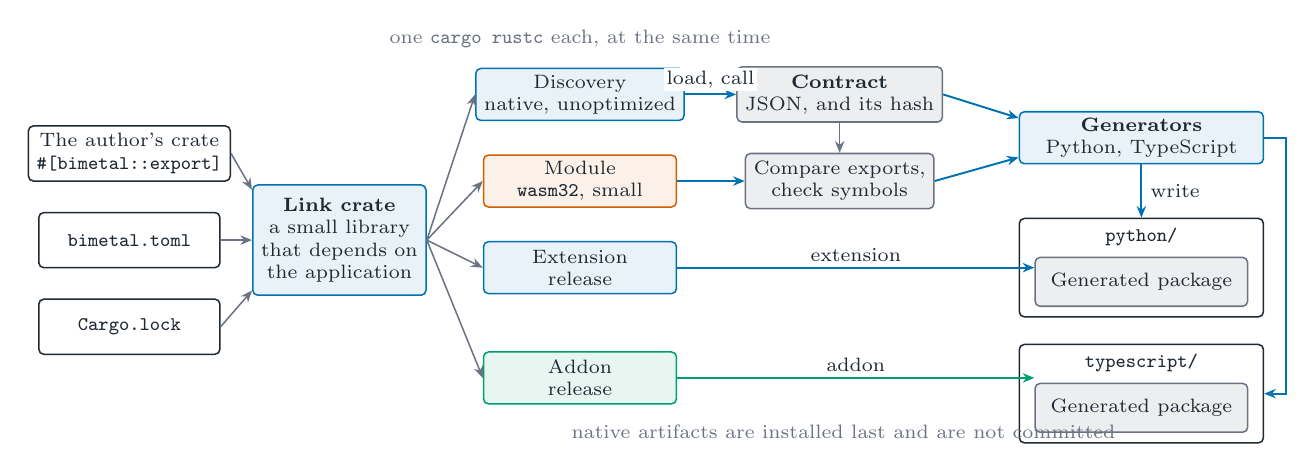
\begin{tikzpicture}[x=0.97cm,y=1cm]
  % The author's files, on the left.
  \node[yours,minimum width=2.3cm] (crate) at (1.25,3.05) {The author's crate\\\ttt{\#[bimetal::export]}};
  \node[yours,minimum width=2.3cm] (toml) at (1.25,1.95) {\ttt{bimetal.toml}};
  \node[yours,minimum width=2.3cm] (lock) at (1.25,0.85) {\ttt{Cargo.lock}};

  % The link crate.
  \node[part,minimum width=1.9cm,minimum height=1.4cm] (link) at (4.0,1.95) {\textbf{Link crate}\\a small library\\that depends on\\the application};
  \draw[plain] (crate.east) -- (link.150);
  \draw[plain] (toml.east) -- (link.west);
  \draw[plain] (lock.east) -- (link.210);

  % The builds, at the same time.
  \node[part,minimum width=2.45cm] (discovery) at (7.15,3.8) {Discovery\\native, unoptimized};
  \node[part,minimum width=2.45cm,draw=wasm,fill=wasm!9] (wasmbuild) at (7.15,2.7) {Module\\\ttt{wasm32}, small};
  \node[part,minimum width=2.45cm] (pybuild) at (7.15,1.6) {Extension\\release};
  \node[part,minimum width=2.45cm,draw=addon,fill=addon!9] (nodebuild) at (7.15,0.2) {Addon\\release};
  \draw[plain] (link.east) -- (discovery.west);
  \draw[plain] (link.east) -- (wasmbuild.west);
  \draw[plain] (link.east) -- (pybuild.west);
  \draw[plain] (link.east) -- (nodebuild.west);
  \node[note] at (7.15,4.5) {one \ttt{cargo rustc} each, at the same time};

  % What discovery gives.
  \node[object,minimum width=2.25cm] (contract) at (10.55,3.8) {\textbf{Contract}\\JSON, and its hash};
  \draw[flow] (discovery.east) -- node[tag,above=1pt] {load, call} (contract.west);
  \node[object,minimum width=2.25cm] (exports) at (10.55,2.7) {Compare exports,\\check symbols};
  \draw[flow] (wasmbuild.east) -- (exports.west);
  \draw[plain] (contract.south) -- (exports.north);

  % The generators, above the projects.
  \node[part,minimum width=3.1cm] (generators) at (14.5,3.25) {\textbf{Generators}\\Python, TypeScript};
  \draw[flow] (contract.east) -- (generators.west |- 0,3.5);
  \draw[flow] (exports.east) -- (generators.west |- 0,3.0);

  % The projects, each with a package inside.
  \node[yours,minimum width=3.1cm,minimum height=1.25cm] (pyproject) at (14.5,1.6) {};
  \node[font=\scriptsize,anchor=north] at (pyproject.north) {\ttt{python/}};
  \node[object,minimum width=2.7cm,minimum height=6.2mm] (pypackage) at (14.5,1.42) {Generated package};
  \node[yours,minimum width=3.1cm,minimum height=1.25cm] (tsproject) at (14.5,0.0) {};
  \node[font=\scriptsize,anchor=north] at (tsproject.north) {\ttt{typescript/}};
  \node[object,minimum width=2.7cm,minimum height=6.2mm] (tspackage) at (14.5,-0.18) {Generated package};
  \draw[flow] (generators.south) -- node[tag,right=2pt] {write} (pyproject.north);
  \draw[flow] (generators.east) -- ++(0.28,0) |- (tsproject.east);

  % Native artifacts skip the generators.
  \draw[flow] (pybuild.east) -- node[tag,above=1pt] {extension} (pypackage.west |- pybuild.east);
  \draw[flow,draw=addon] (nodebuild.east) -- node[tag,above=1pt] {addon} (tspackage.west |- nodebuild.east);
  \node[note] at (10.6,-0.48) {native artifacts are installed last and are not committed};
\end{tikzpicture}

\Description{A left-to-right pipeline: the author's crate, bimetal.toml and Cargo.lock feed a link crate, which compiles up to three of four possible builds. The discovery build yields the contract, the module's build is compared with it, and generators write packages into the Python and TypeScript projects. The extension and the addon are installed directly into the projects.}
\caption{A build. White boxes are the author's files, gray boxes are outputs, and coloured boxes are steps. The discovery build always runs, the extension's build runs when Python is enabled, and the application's choice of JavaScript host selects either the module's build or the addon's.}
\label{fig:pipeline}
\end{figure*}

Four Rust crates implement this design: \ttt{bimetal} is the runtime that applications depend on, \ttt{bimetal-macros} contains the derives and the \ttt{export} attribute, \ttt{bimetal-ir} defines the contract and the naming rules, and \ttt{bimetal-cli} is the command. The command depends on \ttt{bimetal-ir} and never on \ttt{bimetal}, because a command that linked the runtime would also link PyO3 and would then need libpython. For the same reason, the runtime's \ttt{python} feature is off except in the extension's build, so an application's own test binaries do not link libpython either.

\section{The Contract}
\label{sec:contract}

\subsection{Reading the Contract from Compiled Code}

Each marked item expands to code that registers a description of the item with \ttt{inventory}~\cite{inventory}. That crate uses linker constructors, which let one macro expanded in many crates add to a single registry without a central list. The discovery build exists to run this registration and to return its result.

To read the contract, the command loads the discovery build as a library and calls a function named \ttt{bimetal\_\allowbreak discovery\_\allowbreak v1\_\allowbreak contract\_\_\allowbreak \{link package\}}. The function returns a status and a C string, which holds the contract as JSON, a validation error or a panic's message. It catches panics, because a panic that unwound into the command through a C interface would abort the process. Once the command has read the string, it passes the string to a matching \ttt{free} function, which releases it. Appendix~\ref{app:contract} gives the format of the JSON.

The discovery build uses the release profile, with optimization off, incremental compilation on and debug information off. These settings keep it cheap to rebuild, and the release profile gives it the same \ttt{cfg(debug\_assertions)} as the extension. The extra build costs time, and in exchange it provides three properties. First, the contract describes what the compiler built, including the effects of \ttt{cfg} attributes, macros and build scripts. Second, the macros reject a type that the contract cannot represent during the build, with an error that names the Rust item. Third, a macro that generates exports needs no special support, because the discovery build runs after macro expansion.

\subsection{Agreement with What Was Compiled}

The contract comes from one build for the current machine, but a package runs an artifact from another build: a module, an extension or an addon. Four checks make each artifact agree with the contract.

\begin{description}
\item[C1, native hosts.] The extension and the addon are built from the same sources and for the same target as the discovery build, with the runtime's host feature and a different profile. Each artifact computes a hash of its contract when it loads, and the generated code compares this hash with its own. A mismatch raises an error that says to rebuild.
\item[C2, the module's exports.] The module is built for a different compilation target. After this build, the command reads the module's export section. The command stops if the module lacks a function, resource, factory or method of the contract, or has a function or resource that the contract lacks.
\item[C3, unresolved symbols.] If the module needs a symbol that nothing defines, the command stops and names the symbol. A C library compiled for the wrong target usually causes this failure.
\item[C4, conditional exports.] A \ttt{\#[cfg]} attribute on an exported method may test only features, joined by \ttt{all}, \ttt{any} and \ttt{not}, because every build compiles the default features of the application's packages, while the module is built for another target. A test of the target is a compile error, which says to put the condition inside the method's body. A \ttt{cfg} that a \ttt{cfg\_attr} adds, at any depth, is also a compile error, because rustc would remove the method after the macro had listed it, and so is an empty \ttt{any()}, which holds in no build. A gated method is therefore in every artifact or in none, and C1 and C2 check that this holds. Rust evaluates a \ttt{\#[cfg]} on a function or an \ttt{impl} block before the macro runs, so there C2 alone finds a difference between the targets, as it does for a feature that only a dependency of one target turns on.
\end{description}

\begin{claim}[Agreement]
\label{clm:agreement}
Under A3, if \ttt{bimetal build} succeeds, each generated call names a function that exists in its host's compiled artifact, with the signature that the generated code expects.
\end{claim}

\begin{proof}[Argument]
For the native hosts, C1 gives the same sources and target as the discovery build, and the hash comparison rejects an artifact whose contract differs. For the module, C2 gives the same names. The types behind one name come from one Rust source, and by A3, no target changes those types.
\end{proof}

The argument depends on A3 because the command cannot detect a difference inside an export between targets. For example, a constant whose value depends on the target takes the current machine's value in every package. The default of a field is read from the compiled library in the same way, and a package builds its contract again when it loads and refuses to load if that contract differs from the one that the build read. A \ttt{Default}, or the function that \ttt{\#[serde(default = "path")]} names, must therefore give the same value on every call, and the build fails when two calls differ.

\subsection{Names}

A signature means the same thing on every host, but its names have to follow each language's conventions. The naming rules live in \ttt{bimetal-ir}, and the macros and both generators share that one implementation. TypeScript functions, methods and parameters use lower camel case, while Python names stay in snake case. When a language cannot use a parameter's name, the generator renames the parameter in that language only. For example, \ttt{class} becomes \ttt{class\_} in TypeScript and \ttt{class\_value} in Python.

The command refuses a name that it cannot make safe, and it reports all such names in one error. It refuses an export named \ttt{then}, for example, because that export would make a TypeScript module a thenable, and \ttt{await import(...)} would then call the export. It also refuses names that the generated package defines itself, and names that collide after renaming. The checks of a language apply only when that language's host is enabled.

\section{One Wrapper Plan}
\label{sec:wrappers}

A \emph{wrapper} is the native function that a host calls. One function plans the wrapper for every host, so each feature has one implementation rather than three. The macros check each exported signature once, for the contract and for every host. The planned wrapper then decodes the arguments, obtains the resource, calls the author's function and converts the result. This plan is the same for synchronous and asynchronous calls, and for free functions and methods. Where hosts differ, the planner calls an interface named \ttt{HostBackend}, and it never branches on the host itself.

Figure~\ref{fig:call} follows one call to \ttt{greet} from the generated code to the author's function and back. The generated code runs first. In Python it passes each argument as it is, and calls again with Pydantic's dump of an argument that the extension cannot read, such as a dictionary that a caller passes for a model, while in TypeScript it checks the outermost type of each argument. The wrapper then decodes each value once and checks its field rules before it calls the author's function. On the way back, the wrapper checks the result's field rules and makes its host value, which in Python is already an instance of each model's class, so the generated code returns it in Python and freezes it in TypeScript. Section~\ref{sec:costs} reports what the generated code costs compared with the wrapper alone.

\begin{figure}[t]
\centering
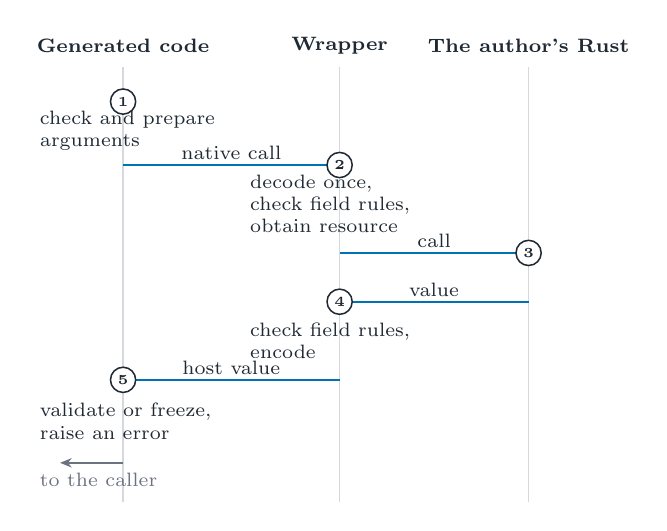
\begin{tikzpicture}[x=1cm,y=0.62cm]
  \tikzset{laneline/.style={draw=rule, line width=0.5pt},
    lanetext/.style={font=\scriptsize, align=left, anchor=west, inner sep=1pt}}
  \def\generated{1.15} \def\wrapper{3.9} \def\user{6.3}
  \node[font=\scriptsize\bfseries,align=center] at (\generated,0.75) {Generated code};
  \node[font=\scriptsize\bfseries,align=center] at (\wrapper,0.75) {Wrapper};
  \node[font=\scriptsize\bfseries,align=center] at (\user,0.75) {The author's Rust};
  \draw[laneline] (\generated,0.3) -- (\generated,-8.6);
  \draw[laneline] (\wrapper,0.3) -- (\wrapper,-8.6);
  \draw[laneline] (\user,0.3) -- (\user,-8.6);

  \node[stepmark] at (\generated,-0.4) {1};
  \node[lanetext] at (0.05,-1.0) {check and prepare\\arguments};
  \draw[flow] (\generated,-1.7) -- node[tag,above=0.5pt] {native call} (\wrapper,-1.7);
  \node[stepmark] at (\wrapper,-1.7) {2};
  \node[lanetext] at (2.72,-2.5) {decode once,\\check field rules,\\obtain resource};
  \draw[flow] (\wrapper,-3.5) -- node[tag,above=0.5pt] {call} (\user,-3.5);
  \node[stepmark] at (\user,-3.5) {3};
  \draw[flow] (\user,-4.5) -- node[tag,above=0.5pt] {value} (\wrapper,-4.5);
  \node[stepmark] at (\wrapper,-4.5) {4};
  \node[lanetext] at (2.72,-5.3) {check field rules,\\encode};
  \draw[flow] (\wrapper,-6.1) -- node[tag,above=0.5pt] {host value} (\generated,-6.1);
  \node[stepmark] at (\generated,-6.1) {5};
  \node[lanetext] at (0.05,-6.95) {validate or freeze,\\raise an error};
  \draw[plain] (\generated,-7.8) -- ++(-0.8,0) node[note,anchor=east,xshift=-1pt] {};
  \node[note,anchor=west] at (0.05,-8.15) {to the caller};
\end{tikzpicture}

\Description{Three vertical lanes, generated code, wrapper and the author's Rust, with five numbered steps of a call moving across them and back.}
\caption{The life of a call. Steps 1 and 5 are generated Python or JavaScript, and steps 2 and 4 are the wrapper.}
\label{fig:call}
\end{figure}

A wrapper for one host compiles only in that host's build, and the application needs no Cargo feature for this. Macro output for the extension passes through \ttt{bimetal::\allowbreak\_\_python\_\allowbreak items!}, which expands its input only when the runtime has its \ttt{python} feature, and \ttt{\_\_node\_\allowbreak items!} does the same for the addon.

A \emph{protocol} is a language feature that a method implements, such as Python's \ttt{len()} or iteration with \ttt{for}. An author requests one with an attribute such as \ttt{\#[bimetal(len)]}. A protocol adds no native code: the macro records it in the contract, a validator checks the method's signature, and the generators write the special members that call the method. For example, \ttt{len(value)} in Python and \ttt{value.length} in TypeScript are generated code around one wrapper.

\section{Values}
\label{sec:values}

How a value crosses depends on how the author writes the signature. Table~\ref{tab:copies} lists the kinds of value, and this section discusses them in three groups: values that are converted field by field, values that cross as one block of memory, and Arrow data.

\begin{table}[t]
\caption{What each host does with a value. A copy here is a copy of the whole payload, and an IPC stream counts as one more copy. Rust's own allocations, such as a \ttt{Vec} that a function returns, are not counted.}
\label{tab:copies}
\small
\begin{tabular}{@{}p{0.17\linewidth}p{0.34\linewidth}p{0.37\linewidth}@{}}
\toprule
Value & Extension & Module and addon \\
\midrule
Model & Read and made as instances of its Pydantic model, field by field & Converted by \ttt{serde-wasm-bindgen} or by the addon's own converter \\
Bytes & One copy each way & One copy each way \\
Buffer & One copy each way & One copy each way \\
Arrow & No copy & An IPC stream and one copy each way \\
Arrow stream & No copy, one batch at a time & An IPC stream and one copy each way, one batch at a time \\
\bottomrule
\end{tabular}
\end{table}

\subsection{Converted Values}

Models, strings, numbers, lists and maps are converted field by field. Serde reads and writes these values through \ttt{pythonize} on the extension, through \ttt{serde-\allowbreak wasm-\allowbreak bindgen} on the module, and through a serializer and a deserializer of our own on the addon. Our deserializer follows \ttt{serde-\allowbreak wasm-\allowbreak bindgen}'s checks, order and error messages, apart from a limit on nesting. In Python, the extension reads an instance of a model's class, a date and a date-time field by field as Python holds them, and it makes a returned model as an instance of its class, as Pydantic would validate it, so neither direction validates a model with Pydantic. A dictionary that a caller passes for a model is the exception, because the extension asks the generated code to call again with Pydantic's dump of it, which Pydantic validates and writes in its JSON mode. A value that holds a numeric buffer goes through Pydantic in both directions, and an argument that holds an enum with data goes through its dump, because the extension cannot read either as Python holds it.

Rust checks an author's field rules on every host. It checks every argument and result of an export, and what a callback returns to Rust, but not the arguments that Rust passes to a callback. The check may look redundant in Python, where Pydantic enforces the same rules when a model is built. However, \ttt{model\_copy(update=...)} skips Pydantic, the extension reads a model instance without it, and TypeScript has no equivalent of Pydantic at all. A returned value that breaks a rule indicates a bug in the Rust code, and the caller then receives an untyped error. A field that is absent holds the Rust \ttt{Default} of its type or what its default function returns, which no caller passed. The model's registration calls that function when the contract is read and checks the value against the field's own rules and the rules inside it, so a default that breaks a rule fails the build. The registration also fails the build when the value holds a NaN or an infinity at any depth, because JSON writes either as \ttt{null}, which inside an \ttt{Option} reads back as \ttt{None}. For the same reason, the derive rejects \ttt{skip\_serializing\_if} on a field with a default function, because Serde would leave out a \ttt{None} and then read the absent field as what the function returns. The derive also checks the \ttt{Default} of a scalar or a list against the field's rules, because it knows that value before the library is compiled.

\subsection{Bytes and Buffers}

Bytes and buffers cross as one block of memory, which avoids the cost of a host object for each element. A \ttt{Vec<u8>}, a slice of bytes or an array of bytes that is a whole parameter or return value crosses as Python \ttt{bytes} or a \ttt{Uint8Array}, while a \ttt{Vec<u8>} field of a model stays a list of integers, as Serde writes it. A \emph{buffer} is the same idea for a numeric array, such as a slice of \ttt{f64}, which reaches the caller as a NumPy array or a typed array. A returned buffer arrives in Python as a \ttt{bytearray}, which NumPy wraps without a further copy.

\subsection{Arrow Values and Streams}

Arrow values show the largest difference between hosts, because only the extension can share their memory with Rust. On the extension, arrays, batches, tables and schemas cross through the PyCapsule interface~\cite{pycapsule}, which is built on the C Data Interface~\cite{arrowc}, without a copy in either direction. The runtime accepts any producer of this interface, after it validates each incoming value. Our tests pass pyarrow values, and one binding crate's test passes a Polars DataFrame. The other two hosts cannot share memory in this way. On the module, a view into WebAssembly memory stops working when the memory grows, and on the addon, the apache-arrow JavaScript library has no C Data Interface. Arrow values on these two hosts therefore cross as an IPC stream, with one copy into Rust's memory and one copy out.

A \emph{stream} of record batches crosses one batch at a time. An export can return a \ttt{Record\allowbreak Batch\allowbreak Stream}, which wraps an asynchronous Rust stream or a blocking reader. Python receives it as a pyarrow \ttt{Record\allowbreak Batch\allowbreak Reader}, which is built on the C Stream Interface~\cite{arrowc}, and any thread can ask this reader for the next batch, including the worker threads of a query engine such as DuckDB. A parameter can also take a stream, from any producer of the interface, and the runtime then reads each batch only when the Rust code asks for it. A synchronous export reads on its caller's thread, while an asynchronous export, which starts on the runtime because it takes a stream, reads each batch on a blocking thread of the runtime and never on a worker. Dropping a stream drops its source, which cancels the source's work. The first error ends a returned stream: every later read fails with the same message, and a typed error keeps its code at the start of that message.

On the module and the addon, TypeScript reads a returned stream as an asynchronous iterator, and each batch crosses as its own IPC stream. In the other direction, a JavaScript source writes a batch only when Rust asks for one. JavaScript makes these batches asynchronously, and a synchronous call on its one thread could not wait for them. The command therefore refuses a stream parameter of a synchronous export when an application builds a TypeScript package.

\begin{claim}[Streams without the lock]
\label{clm:stream}
Rust never waits for a batch of a stream parameter while it holds the interpreter lock. A returned stream releases the lock before it waits for a batch.
\end{claim}

\begin{proof}[Argument]
A synchronous export that takes a stream runs without the lock, because the macros refuse a brief export, which keeps the lock, when it takes a stream or a callback, so it reads its parameter's batches without the lock. An asynchronous export with a stream parameter runs on the runtime's workers, which never hold the lock, and it reads each batch on a blocking thread. A read of a returned stream checks whether its thread holds the lock. If the thread holds it, the read releases it, waits for the batch and takes the lock back.
\end{proof}

This claim matters because a source may need the lock to make its next batch, as a pyarrow reader over a Python generator does, or a stream that calls a Python function. If a read waited with the lock held, the source would wait for the read, and neither would finish. One test covers this case: a Python function feeds a returned stream, and an import that holds the lock reads the stream. Without the release, that test does not finish.

Two further rules apply to Arrow. First, streams do not survive a fork. Once the runtime has started, a forked child cannot read a stream that its parent returned: every read fails in the child, and the child never drops the stream, because the stream may hold tasks of the parent's runtime. Second, an application's Arrow values must have the same Rust types as the Arrow crate that the application already uses, and Rust treats two versions of one crate as different types. The runtime therefore has an \ttt{arrow} feature for arrow-rs 60 and an \ttt{arrow-59} feature for arrow-rs 59. Each feature names its crates the same way at the crate root, which gives the runtime one code path for both versions. A version range would not work, because Cargo keeps both versions and gives each dependent the highest one it allows.

\section{Resources}
\label{sec:resources}

A resource must keep three of Rust's guarantees after a caller in another language holds a reference to it: no reader sees a value during a write, no call uses a freed value, and a method that takes \ttt{\&mut self} has exclusive access. To provide these guarantees, every resource keeps its value in one structure named \ttt{Resource}, which holds a shared cell around an \ttt{Arc} of a Tokio read-write lock. Seven rules govern this structure.

\begin{description}
\item[R1, obtaining.] A call clones the \ttt{Arc} when it starts. This means that a call keeps the value alive even after the resource is closed (R3), and Rust drops the value after the last call ends.
\item[R2, locking.] A \ttt{\&self} method takes the read lock, and a \ttt{\&mut self} method takes the write lock. Each keeps its lock until its result has been converted, except an asynchronous method on the extension, which releases its lock when its Rust call returns, because its result converts on the thread where a synchronous call waits for the lock.
\item[R3, closing.] \ttt{close()} empties the shared cell without waiting for running calls. If no call has a clone, Rust drops the value inside \ttt{close()}, on the calling thread. A later call fails with an error that names the method.
\item[R4, taking.] A \ttt{self} method or a parameter of type \ttt{T} moves the value out and closes the resource. This succeeds only if no other call has a clone. If a call fails after it took a \ttt{T} argument, the resource stays closed and its value is gone.
\item[R5, one use in a call.] If a call receives one resource twice, in two parameters or as its receiver and a parameter, the call fails.
\item[R6, thread safety.] When Python is enabled, a resource's type must be \ttt{Send} and \ttt{Sync}. The compiler checks this bound when it builds the extension.
\item[R7, inside a callback.] While a thread runs a function that a \ttt{bimetal::Callback} called, a synchronous call on that thread does not wait for a lock. If the lock is taken, the call fails with an error that says the resource is busy.
\end{description}

\begin{claim}[Aliasing]
\label{clm:aliasing}
A caller cannot use a freed resource. While one call has \ttt{\&mut T}, no other call has any reference to that \ttt{T}.
\end{claim}

\begin{proof}[Argument]
By R1, a call obtains the value only through a clone of the \ttt{Arc}, and that clone keeps the value alive. By R3 and R4, a call that starts after a close or a move finds the cell empty. By R2, the read-write lock makes a \ttt{\&mut T} exclusive. By R4, a move succeeds only when no other call has a clone. \ttt{Resource} and the code that the macros emit use no \ttt{unsafe} code. On the addon, the runtime reads the object behind a method's receiver or an argument through \ttt{napi\_unwrap} and one unchecked dereference, after a type-tag check. Rust's type system guarantees the remaining cases~\cite{matsakis2014rust}.
\end{proof}

\begin{claim}[No waiting for itself]
\label{clm:self}
A call cannot wait for itself through its receiver, its arguments or a callback.
\end{claim}

\begin{proof}[Argument]
A call could wait for itself in two ways. First, it could take one resource's lock twice. By R5, such a call fails before it takes the second lock. Second, a function that the call runs through a callback could make a synchronous call that needs a lock the outer call holds. By R7, this inner call fails and does not wait. The function then raises an exception, and the outer call receives it as an error value.
\end{proof}

R7 is what makes this argument hold on the extension, the one host where a synchronous call can wait. Suppose a synchronous \ttt{\&self} method $a$ calls a Python function, and that function calls a \ttt{\&mut self} method $b$ of the same resource. Without R7, $b$ would wait for $a$'s read lock while $a$ waited for the function to return, and neither would finish. With R7, $b$ fails at once, although a read inside the same function succeeds, because readers share the lock. The rule has a cost: if the function calls a different resource while another thread is using it, that call also fails, as a synchronous call in JavaScript does. The rule cannot be narrower, because a thread cannot tell which call holds a lock.

Two cases fall outside Claim~\ref{clm:self}. In the first, call $a$ takes resource $x$ and then waits for $y$, while call $b$ takes $y$ and then waits for $x$. These two calls wait for each other, as the holders of any two locks can. Bimetal does not order locks globally, because an author's Rust code would then have to know about the order. In the second, the function that a callback runs starts a thread of its own and waits for it. R7 applies only to the thread that runs the function, so a call on the new thread can still wait for the outer call.

\subsection{What a Host Does with a Busy Resource}

A resource is \emph{busy} when a call needs a lock that conflicts with one that another call holds. The hosts cannot all offer the same behaviour for a busy resource, and Table~\ref{tab:busy} lists what each one does. To see why they differ, suppose a caller starts an asynchronous call $a$ to a \ttt{\&mut self} method, and $a$ takes the write lock. Before $a$ finishes, the caller makes a synchronous call $b$ to the same resource on the same thread. In JavaScript, $b$ throws an error, because the code that would finish $a$ could never run while $b$ waited on the one thread. In Python, $b$ waits and releases the interpreter lock, so other Python threads keep running. Call $a$ finishes on a Tokio thread, and $b$ then continues. If $b$ runs on the event loop's own thread, however, it blocks that loop while it waits.

\begin{table}[t]
\caption{What a call does when its resource is busy. A \ttt{self} method needs the value alone, and it fails if any other call has a clone.}
\label{tab:busy}
\small
\begin{tabular}{@{}lll@{}}
\toprule
The call & Python & JavaScript \\
\midrule
Sync method & Waits & Throws an error \\
Sync, in a callback & Fails with an error & Throws an error \\
Async method & Waits in its future & Waits in its future \\
\ttt{self} method & Fails with an error & Fails with an error \\
\bottomrule
\end{tabular}
\end{table}

The hosts also differ in when an asynchronous method takes its lock. On the JavaScript hosts, the method tries its lock on the calling thread when the caller makes the call. In Python, this attempt happens when the generated coroutine first runs. A call that gets the lock holds the resource from that moment, even on the module, where the Rust body starts in a later microtask. If the lock is taken, the call waits in its future and joins the lock's queue when its future is first polled. On the native hosts, a multi-threaded runtime makes every poll after the first, so calls that find the lock taken have no guaranteed order among themselves.

\subsection{Blocks and Failure}

Python's \ttt{with} and TypeScript's \ttt{using}~\cite{explicitresource} close a resource when a block ends. If a method is marked \ttt{exit}, it runs first and receives a flag that says whether the block failed. Python passes the real exception state, but JavaScript does not tell the dispose method whether the block threw, so the generated TypeScript always passes \ttt{failed = true}. The consequence shows in a resource whose \ttt{exit} method commits when \ttt{failed} is false and rolls back otherwise: a TypeScript author must commit explicitly before the block ends. If the author forgets, the resource rolls back, which is the safer of the two outcomes.

\subsection{Callbacks}

A parameter of type \ttt{bimetal::Callback<A, R>} holds a Python or JavaScript function that Rust can keep and call from any thread. What happens during that call depends on the host. On the extension, the call takes the interpreter lock, and on the module it runs on the only thread. On the addon, a call on the JavaScript thread runs directly, while a call from another thread hands the work to the JavaScript thread and waits. This last case has a hazard. A synchronous export occupies the JavaScript thread while it runs, so it must not wait for a callback made on another thread, because that callback needs the same thread. The runtime cannot detect this case. The extension has the same hazard for a brief export, which keeps the interpreter lock that a callback on another thread must take, so the macros refuse a brief export that takes a callback or a stream. On every host, if the function raises an exception, Rust receives an error value, which the author maps into a typed error.

\section{Failures}
\label{sec:failures}

A call can fail with a typed error, a bad argument, a panic or a trap, and only the first of these is part of the API. Each Rust error type becomes a class with a \ttt{code} field, and the declared type of that field lists every code, so a type checker catches a misspelled one. A bad argument raises the language's own error, which names the function and the parameter. Panics and traps are bugs in the Rust code, and the rest of this section concerns them.

A panic must not unwind into a caller, because that would abort the process. On the native hosts, the wrapper catches the panic and reports it. The extension raises \ttt{PanicException}, which derives from \ttt{BaseException} so that \ttt{except Exception} does not hide a bug, and the addon throws an \ttt{Error}. Both hosts stay usable afterwards. A later call can, however, reach a resource whose \ttt{\&mut self} method panicked partway, because Tokio's lock does not record a panic. So that a panic never ends the process, the command builds these artifacts to unwind even when the application's Cargo profile sets \ttt{panic = "abort"}.

The module cannot catch a panic, because in WebAssembly a panic becomes a trap. The trap leaves the module with its memory, locks and asynchronous executor as they were partway through a call. It also leaves every other pending promise waiting for a future that can never finish, so an application would hang with no error. Bimetal therefore wraps every export of the module in a function called the \emph{guard}, which turns a trap into errors. The command changes the code that wasm-bindgen generates, so that every call into the module passes through the guard, including the asynchronous executor's microtasks and the finalizers.

Figure~\ref{fig:trap} shows what happens when a call traps while another call is pending. Suppose a caller starts an asynchronous call $a$. As every asynchronous wrapper does when its call starts, the wrapper for $a$ registers the function that rejects $a$'s promise. The caller then makes a synchronous call $b$, and $b$ panics. The panic hook gives the guard the panic's message, the module traps, and an exception leaves the module. The guard treats any exception from the module as proof of a trap, because Rust returns its errors as values and never throws. It records the abort and rejects $a$'s promise, and call $b$ throws an \ttt{Error} with the panic's message. When the caller later makes a call $c$, the generated code finds the record and throws at once, without entering the module. From this point \ttt{close()} does nothing, so that a \ttt{using} block reports the panic and not a second failure. The process keeps running, and only a reload makes the module callable again.

\begin{figure}[t]
\centering
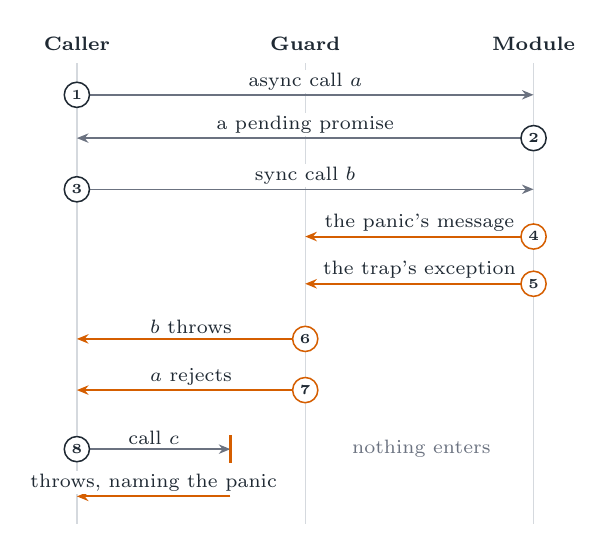
\begin{tikzpicture}[x=1cm,y=0.5cm]
  \tikzset{laneline/.style={draw=rule, line width=0.5pt},
    stepnote/.style={font=\scriptsize, align=center, inner sep=1pt, fill=white}}
  \def\caller{0.7} \def\guard{3.6} \def\module{6.5}
  \node[font=\scriptsize\bfseries] at (\caller,0.8) {Caller};
  \node[font=\scriptsize\bfseries] at (\guard,0.8) {Guard};
  \node[font=\scriptsize\bfseries] at (\module,0.8) {Module};
  \draw[laneline] (\caller,0.3) -- (\caller,-11.4);
  \draw[laneline] (\guard,0.3) -- (\guard,-11.4);
  \draw[laneline] (\module,0.3) -- (\module,-11.4);

  \draw[plain] (\caller,-0.5) -- node[stepnote,above=0.5pt] {async call $a$} (\module,-0.5);
  \node[stepmark] at (\caller,-0.5) {1};
  \draw[plain] (\module,-1.6) -- node[stepnote,above=0.5pt] {a pending promise} (\caller,-1.6);
  \node[stepmark] at (\module,-1.6) {2};
  \draw[plain] (\caller,-2.9) -- node[stepnote,above=0.5pt] {sync call $b$} (\module,-2.9);
  \node[stepmark] at (\caller,-2.9) {3};
  \draw[flow,draw=wasm] (\module,-4.1) -- node[stepnote,above=0.5pt] {the panic's message} (\guard,-4.1);
  \node[stepmark,draw=wasm] at (\module,-4.1) {4};
  \draw[flow,draw=wasm] (\module,-5.3) -- node[stepnote,above=0.5pt] {the trap's exception} (\guard,-5.3);
  \node[stepmark,draw=wasm] at (\module,-5.3) {5};
  \draw[flow,draw=wasm] (\guard,-6.7) -- node[stepnote,above=0.5pt] {$b$ throws} (\caller,-6.7);
  \node[stepmark,draw=wasm] at (\guard,-6.7) {6};
  \draw[flow,draw=wasm] (\guard,-8.0) -- node[stepnote,above=0.5pt] {$a$ rejects} (\caller,-8.0);
  \node[stepmark,draw=wasm] at (\guard,-8.0) {7};
  \draw[plain] (\caller,-9.5) -- node[stepnote,above=0.5pt] {call $c$} (2.65,-9.5);
  \node[stepmark] at (\caller,-9.5) {8};
  \draw[wasm,line width=0.9pt] (2.65,-9.85) -- (2.65,-9.15);
  \draw[flow,draw=wasm] (2.65,-10.7) -- node[stepnote,above=0.5pt] {throws, naming the panic} (\caller,-10.7);
  \node[note,anchor=west] at (4.15,-9.5) {nothing enters};
\end{tikzpicture}

\Description{A sequence diagram with a caller, the guard and the module, in eight numbered steps. Call a is pending when call b panics; the guard rejects a, b throws, and a later call c never enters the module.}
\caption{A trap, read from top to bottom. Without the guard, call $a$'s promise in step 7 would stay pending for ever, and call $c$ in step 8 would enter a module in an unknown state.}
\label{fig:trap}
\end{figure}

\begin{claim}[Trap]
\label{clm:trap}
After a trap, no call enters the module, and no promise that depends on the module stays pending.
\end{claim}

\begin{proof}[Argument]
Every path into the module passes through the guard. When the guard sees a trap, it records the abort and rejects the pending promises. It then rethrows to a wrapper's call, or returns from an outermost microtask or finalizer, whose exception no caller could catch. The generated code checks the record before it enters the module, and the guard checks it again. Each asynchronous wrapper registers its promise's rejection when its call starts, and the guard rejects all of them. A callback can call back into the module, and that inner call can trap. The callback then fails, Rust receives this failure as an error value, and the outer call could return normally from an unusable module. The guard therefore throws when the outermost call returns.
\end{proof}

\section{Async}
\label{sec:async}

An \ttt{async fn} becomes a Python coroutine and a TypeScript function that returns a \ttt{Promise}, and the host decides what runs it. The native hosts run these futures on a Tokio runtime that the process starts on demand, while the module runs them on the JavaScript event loop.

A native host polls a future once on the caller's thread before it gives the future to the runtime, because a call that finishes without a wait, such as a read from memory, then needs no worker. Such a call settles its asyncio future or its promise at once, while a call that waits becomes a task of the runtime, whose first poll replaces the waker of the caller's poll. That first waker wakes no one, so a future must register its waker on every poll, and code before the first wait runs outside any Tokio task. The extension makes that first poll without the interpreter lock, as it runs a synchronous export, so work before the first wait stops the caller's event loop but no other Python thread.

Long work on the caller's thread would stop its event loop, and the calls of one loop would then run one after another on one core, so each asynchronous export keeps a \emph{pace}. The pace is a running average of the time that the export's calls spend in their polls, together with the number of its calls that run on workers, and each timed call updates it. A call starts on a worker when its export works for more than 2.5 times the cost of a hand-off to a worker, so that the hand-off adds at most 40\% to the work that it moves, or for more than one hand-off while other calls of the export run on workers, so that concurrent calls spread over cores. We take that cost to be 25~$\mu$s, which is near what Section~\ref{sec:costs} measures for a call that waits once. Timing a call reads the clock twice, so a call of an export that works briefly times itself only once in eight calls, while every call of an export that works longer times itself, and so does the call after a long one. A call counts as the lesser of its own time and that of the last timed call, because the scheduler can stall any thread, and one stalled call must not move the export's later calls to workers. An export whose calls turn slow therefore moves after two long calls in a row when each takes more than four times the limit, and after more calls when they are shorter, because each counted call moves the average a quarter of the way. Until then, its calls run on the caller's thread.

A call that takes a \ttt{Callback} or a \ttt{Record\allowbreak Batch\allowbreak Stream} is the exception, and a worker makes its first poll, because such a call may wait for the caller's event loop before its first wait. A Python function may wait for a coroutine on that loop, and on the addon JavaScript writes a stream argument on the thread that runs the loop. On the caller's thread, either wait would never end. The macros know the type of each parameter, so they choose where each asynchronous export starts when they expand it.

On the extension, a worker thread must be able to finish a call without waiting for the interpreter lock. The asyncio future is therefore kept in a structure that only code holding that lock can touch. A \ttt{Callback} argument is the exception, because the task owns its Python function, and if the last clone drops on a worker thread, PyO3 defers the release to its reference pool. When the task finishes, the worker posts the call to its event loop's \emph{mailbox}, and it wakes the loop only when the mailbox was empty. On Unix, the loop watches one end of a socket pair, and the worker writes a byte to the other end without the interpreter lock, so a result reaches the loop with one wake-up. The loop then converts every result in the mailbox and settles each future, so calls that finish together settle in one turn of the loop and take the lock once. A loop that cannot watch a socket, such as the proactor loop on Windows, is woken instead by a blocking thread that takes the lock and schedules the mailbox, once for each batch. A mailbox belongs to the process that made it, so a forked child leaks the parent's mailboxes, whose locks a worker of the parent may have held at the fork. The addon delivers results in the same way through its \emph{courier}, a single thread-safe function of each environment, which Node.js drains, up to 999 jobs at a time, when its event loop wakes, so neither a call that waits nor a callback argument creates a thread-safe function of its own. Cancellation works in Python only. When a caller cancels the future, a callback aborts the task, and Tokio drops the Rust future at its next opportunity. A JavaScript promise cannot be cancelled, so a call there runs to its end.

Some synchronous calls also run inside the Tokio runtime: constructors, factories, and functions and methods that return a resource, because a resource may need to spawn tasks that it keeps. Other synchronous calls do not run inside it, and a package with no resources or asynchronous calls never starts a thread. A child process created by \ttt{fork} starts its own runtime, because the parent's worker threads do not exist in the child. Calls that were running in the parent do not continue in the child, and cancelling one there does nothing. If one of those calls held a resource, the resource stays held in the child, and a call there that needs it waits for ever.

The module has no Tokio runtime, so an author whose code uses Tokio's I/O, timers or \ttt{spawn} needs another implementation for that target. A library that spawns tasks internally, as DataFusion does, can still run on a single-threaded runtime of its own through \ttt{block\_on}, as long as nothing it awaits needs I/O or a timer.

\section{Reproducible Output}
\label{sec:reproducible}

An application commits its module and generated source, and \ttt{bimetal check --rebuild} compiles them again and compares the bytes. This comparison is useful only if two machines produce the same bytes~\cite{lamb2022reproducible}. By default they do not, because absolute paths reach the output in two ways.

The first way is through panic messages, which name source files and are part of the module. The command therefore remaps every local path in every compilation for a build's target. The workspace's files become relative paths, the Cargo home becomes \ttt{/cargo}, the target directory becomes \ttt{/target}, and the link crates become \ttt{/bimetal-link}. Packages outside the workspace become \ttt{/source/\{name\}}, and the standard library's sources become \ttt{/rustc/\{commit\}}. Diagnostics map these paths back, so an author still sees the real ones.

The second way is through each crate's identity, which comes from rustc's \ttt{-C metadata} flag. This identity appears in symbol names, decides the order of the module's functions and is part of every \ttt{TypeId}. Cargo hashes into this flag the absolute path of each local package that lies outside the workspace being built. The link crate lies outside the application's workspace, so the application's packages are among these local packages. For build scripts and procedural macros, Cargo also hashes in the build machine's target triple. The command therefore runs rustc through a small program of its own, which replaces the flag with a hash of the package's remapped directory, the crate's name and crate types, and its \ttt{--cfg} flags.

Lastly, the command strips the module's \ttt{name} and \ttt{producers} custom sections, which contain debug names and toolchain metadata.

\begin{claim}[Reproducibility]
\label{clm:reproducible}
Under A1 and A2, two checkouts of one commit, at any path, on Linux or macOS, with one toolchain, produce the same module and the same generated sources.
\end{claim}

We support this claim with tests rather than a proof. Continuous integration rebuilds the committed examples on Linux and macOS, on machines that did not build them, and compares the bytes. The claim excludes Windows, because rustc keeps Windows separators in the part of a path after the remapped prefix, and those separators reach the module through panic messages. A committed module should therefore come from another platform.

\subsection{A Fingerprint That Stays Equal}

To avoid compiling when nothing changed, the command records a fingerprint of a build's inputs. This fingerprint is committed, so it must not differ between machines: if it covered anything specific to one machine, a build on another machine would change a committed file. The command therefore divides what a build read into two groups (Figure~\ref{fig:inputs}). The inputs that every checkout has are hashed into the \emph{source fingerprint} in \ttt{bimetal.toml}. The command assumes that every checkout of a commit has the files among them, which are the files that \ttt{.gitignore} does not exclude. Every other input is a \emph{local input}, and the command records these in an ignored file.

\begin{figure}[t]
\centering
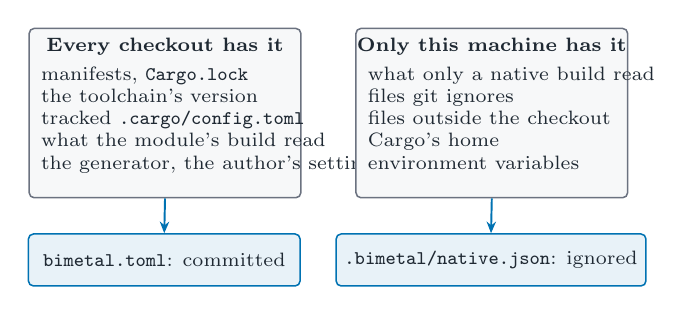
\begin{tikzpicture}[x=1cm,y=1cm]
  \node[object,minimum width=3.45cm,minimum height=2.15cm,fill=rule!18,anchor=north west] (checkout) at (0,0) {};
  \node[font=\scriptsize\bfseries,anchor=north,align=center] at (checkout.north) {Every checkout has it};
  \node[font=\scriptsize,anchor=north west,align=left,inner sep=2pt] at (0.08,-0.42) {manifests, \ttt{Cargo.lock}\\the toolchain's version\\tracked \ttt{.cargo/config.toml}\\what the module's build read\\the generator, the author's settings};
  \node[object,minimum width=3.45cm,minimum height=2.15cm,fill=rule!18,anchor=north west] (machine) at (4.15,0) {};
  \node[font=\scriptsize\bfseries,anchor=north,align=center] at (machine.north) {Only this machine has it};
  \node[font=\scriptsize,anchor=north west,align=left,inner sep=2pt] at (4.23,-0.42) {what only a native build read\\files git ignores\\files outside the checkout\\Cargo's home\\environment variables};
  \node[part,minimum width=3.45cm] (toml) at (1.725,-2.95) {\ttt{bimetal.toml}: committed};
  \node[part,minimum width=3.45cm] (native) at (5.875,-2.95) {\ttt{.bimetal/native.json}: ignored};
  \draw[flow] (checkout.south) -- (toml.north);
  \draw[flow] (machine.south) -- (native.north);
\end{tikzpicture}

\Description{Two boxes of build inputs. Those every checkout has go to bimetal.toml, and those only this machine has go to .bimetal/native.json.}
\caption{Where a build's inputs are recorded. The module's build reads the same files on every machine, and its list of inputs is therefore the same on each machine.}
\label{fig:inputs}
\end{figure}

The generator itself is one of the inputs in the first group. The command's build script hashes the generator's own sources into the source fingerprint, so a change to the generator rebuilds applications even when the version number stays the same. If an application has no module, the command records what the discovery build read instead. That list is the same on every machine only while no code compiled for one operating system alone reads a file. A1 applies here too, because the command cannot detect what a build script reads without telling Cargo.

\subsection{Ownership of Files}

A generator that writes into a project must not destroy an author's work. The command therefore records every file that it writes, and it writes only inside the package folder. Before it changes anything, it stops if a new path would overwrite a file that it does not own. It then copies each changed file through a temporary file beside the destination, deletes its own stale files, and updates \ttt{bimetal.toml} last. If a build stops midway, the project contains only the command's files beside the author's, and the next build adopts them. A file whose bytes did not change keeps its modification time, so a file watcher does not run again.

\section{Testing}
\label{sec:testing}

Bimetal's promises concern what a caller sees, so most of its tests build real packages and call them from real runtimes. An example application called \ttt{showcase} uses every feature except \ttt{arrow-59}, and its tests run on all three hosts. A second example returns and takes streams, and its tests read and pass them with pyarrow, DuckDB and Polars. Every test file runs on the addon unless a short list marks it as specific to the module, so a new file is tested on the addon by default. The Python tests also run \ttt{mypy --strict} and strict pyright on the generated package, and the TypeScript tests type-check against the generated declarations. Finally, each package is built as a wheel or a tarball, installed into a new project outside the repository, and loaded there.

Below this level, unit tests cover the naming rules, the fingerprints and the writing of files, and a set of compile-fail tests checks the macros' error messages. The runtime's own tests embed CPython to drive asynchronous calls with asyncio and to test \ttt{fork}. A further test requires every Rust, Python and TypeScript sample in the documentation to appear in a program that runs.

To learn what real code needs, we also wrote binding crates for five large Rust projects: DataFusion, Oxc, Polars, Tantivy and Typst, which range from about 134,000 to about 575,000 lines of Rust. Each binding crate is a few hundred lines. We wrote each API as a user of that project would want it, before we checked what Bimetal allowed. This work led to most of the features in Section~\ref{sec:resources}, including resources returned from methods, callbacks and \ttt{exit}.

\section{What It Costs}
\label{sec:costs}

Bimetal has three kinds of cost: time on every call, memory for copies, and time to build. We measure the first with a \emph{crossing lab}, which builds a probe application with one export for each kind of value and call, and times each crossing on each host. The lab can also build an earlier version of Bimetal and run the two builds in turns, one process of each per round, so that a change in the machine's load reaches both, and a change to the runtime is measured against the version before it. Table~\ref{tab:costs} gives its measurements on an Apple M5 laptop with 10 cores and 32~GiB of memory, on macOS 27, with Rust 1.94, Python 3.11 and Node.js 24. Each cell is the median of ten rounds, and each round's figure is the median of fifteen samples of about a millisecond of calls. These numbers show where the costs are, and they do not compare Bimetal with other tools.

\begin{table}[t]
\caption{Median time per call into the probe. ``Native only'' calls the function that the wrapper calls, with the arguments that the wrapper passes. A \ttt{Row} model has six fields, among them a list and a date. The rows of 32 calls at once give the time per call while 32 calls run together, and in the last row each call works for about 170~$\mu$s without waiting.}
\label{tab:costs}
\small
\setlength{\tabcolsep}{4pt}
\begin{tabular}{@{}lrrr@{}}
\toprule
Call & Extension & Module & Addon \\
\midrule
No arguments & 52~ns & 46~ns & 24~ns \\
\quad Native only & 41~ns & 34~ns & 21~ns \\
100 integers out & 475~ns & 2.4~$\mu$s & 1.3~$\mu$s \\
100 \ttt{Row} models in & 35.0~$\mu$s & 88.1~$\mu$s & 67.2~$\mu$s \\
\quad Native only & 34.5~$\mu$s & 78.8~$\mu$s & 59.7~$\mu$s \\
100 \ttt{Row} models out & 46.6~$\mu$s & 96.2~$\mu$s & 35.8~$\mu$s \\
\quad Native only & 46.0~$\mu$s & 81.9~$\mu$s & 34.9~$\mu$s \\
1~MiB of bytes & 48~$\mu$s & 430~$\mu$s & 104~$\mu$s \\
One Arrow row out & 2.4~$\mu$s & 31~$\mu$s & 28~$\mu$s \\
Async, no wait & 0.29~$\mu$s & 0.63~$\mu$s & 0.23~$\mu$s \\
Async, one yield & 22.5~$\mu$s & 0.66~$\mu$s & 10.0~$\mu$s \\
\quad 32 calls at once & 5.2~$\mu$s & 0.65~$\mu$s & 1.6~$\mu$s \\
Async, long work, 32 at once & 29.9~$\mu$s & 173~$\mu$s & 27.3~$\mu$s \\
\bottomrule
\end{tabular}
\end{table}

The table shows four things. First, a Python call with models costs about what its native function costs, because the extension reads a model instance and makes a returned model itself, so 100 \ttt{Row} models in cost 35.0~$\mu$s, of which the native function takes 34.5~$\mu$s, and 100 integers out cost 475~ns, of which the wrapper's code takes 45~ns. The addon makes each object of a result with one call into JavaScript, so 100 models out cost 35.8~$\mu$s there, while the module converts each value through \ttt{serde-\allowbreak wasm-\allowbreak bindgen}. A brief call keeps the interpreter lock, so a call with no arguments costs 18~ns on the extension instead of 52~ns. Second, an Arrow value costs little on the extension, where it crosses through the C Data Interface, while on the JavaScript hosts the IPC stream that apache-arrow reads and writes costs most of the call. Third, an asynchronous call that waits once costs more on the native hosts than on the module, because the yield moves the call to a worker thread and its result back, which is two wake-ups of a thread. On the extension, a Python thread that hands a future to another Python thread and back takes 19.7~$\mu$s on the same machine, so the call costs little more than Python itself. Calls that finish together settle in one turn of the event loop, so 32 calls at once cost 5.2~$\mu$s each on the extension. Fourth, 32 calls that each work for 170~$\mu$s without waiting cost 29.9~$\mu$s each on the extension and 27.3~$\mu$s on the addon, because their export's pace starts them on workers, while the module, which has one thread, runs them one after another.

Against the release before these changes, measured in turns by the lab on the same machine while other work loaded it, a call with 100 \ttt{Row} models out took 0.37 times as long on the extension, 0.59 times on the module and 0.22 times on the addon, and a call with 100 models in took 0.32, 0.57 and 0.53 times as long. On the extension, a callback took 0.18 times as long, and 32 waiting calls at once took 0.24 times as long, or 0.55 times with another Python thread competing for the interpreter lock, because each of those calls still releases the lock, and taking it back waits for the other thread. The 32 calls of long work took 0.19 times as long on both native hosts.

We also measured peak memory, to check the copies in Table~\ref{tab:copies}. When a call reversed 100~MiB of bytes, peak memory rose by 3.0 times the payload on every host: one copy in, Rust's result and one copy out. When an Arrow call passed 16~MB, peak memory rose by 0.06 times the payload on the extension and by about 4.1 times the payload on the JavaScript hosts, which is one stream and one copy in each direction.

Build time is the third cost. A first build compiles every dependency once for each host, which took 14 to 42 seconds for three of our small examples and several minutes for each of the five large projects. A build where nothing changed took 70 to 88 milliseconds, and \ttt{bimetal check} took about the same.

\section{Limitations}
\label{sec:limitations}

\emph{The arguments in this paper are informal.} The claims rest on the code and on the tests that exercise it. There is no machine-checked model, and the claims do not cover bugs in PyO3, wasm-bindgen, Node-API or the compiler.

\emph{Three interfaces need \ttt{unsafe} code.} These are Node-API's calls, the C Data Interface and the discovery interface. Tests and code review check this code, and the tests do not run under a sanitizer or Miri.

\emph{Checks cost time on every call.} Rust checks the field rules of every argument and result, whether or not a caller needs it, and a caller cannot turn this off. Each call also runs generated code, unless a Python export is brief and passes its values on as they are, and in Python a value that holds a numeric buffer goes through Pydantic in both directions.

\emph{The contract has gaps.} The command does not enforce A3 inside an export. Bimetal does not support untagged or adjacently tagged enums, tuple variants that hold other than one value, \ttt{\#[serde(flatten)]}, generic types, \ttt{u128}, maps with keys other than strings, bytes inside a model, keyword-only arguments or asynchronous callbacks. In TypeScript, only an asynchronous export can take a stream of record batches.

\emph{Each host costs its own build.} When a project is large, a first build takes minutes and gigabytes, because every dependency compiles once for each host.

\section{Related Work}
\label{sec:related}

Table~\ref{tab:related} compares Bimetal with the closest tools, as their own documentation described them on 6 November 2026. PyO3, napi-rs and wasm-bindgen each give an author full control of one runtime, and Bimetal uses PyO3, wasm-bindgen and napi-rs's low-level \ttt{napi-sys} crate underneath. These tools trade repeated work for a result shaped exactly to one runtime. UniFFI and Diplomat generate bindings for many languages from one definition, and they cover far more languages than Bimetal does. In exchange, Bimetal offers Pydantic models, Arrow without a copy in Python, and \ttt{async} and protocols in both of its languages.

\begin{table}[t]
\caption{Tools closest to Bimetal.}
\label{tab:related}
\footnotesize
\setlength{\tabcolsep}{3pt}
\begin{tabular}{@{}p{0.25\linewidth}p{0.32\linewidth}p{0.2\linewidth}p{0.16\linewidth}@{}}
\toprule
Tool & Runs in & Definition & Types for callers \\
\midrule
Bimetal & Python, Node.js, browsers & Compiled Rust & Generated \\
PyO3~\cite{pyo3}, maturin~\cite{maturin} & Python & Rust macros & By hand by default \\
napi-rs~\cite{napirs} & Node.js & Rust macros & Generated \\
wasm-bindgen~\cite{wasmbindgen} & Browsers, Node.js & Rust macros & Generated \\
UniFFI~\cite{uniffi} & Kotlin, Swift, Python, Ruby, others & Macros or a file & Generated \\
Diplomat~\cite{diplomat} & C, C++, Dart, JavaScript, .NET, Kotlin, Python & A bridge module & Generated \\
\bottomrule
\end{tabular}
\end{table}

Earlier generators read a definition that is separate from the compiled code. SWIG~\cite{beazley1996swig} generates bindings from C and C++ headers, and Thrift~\cite{slee2007thrift} generates them from an interface definition language. Bimetal reads the definition from compiled code instead, so the definition matches what the compiler built for the discovery build, and C1 to C4 and A3 cover the other builds. Other work checks or removes the boundary rather than generating it. Furr and Foster check foreign calls statically against the host language's types~\cite{furr2005}, and Jeannie lets a program mix Java and C in one file and generates the boundary~\cite{hirzel2007jeannie}. Grimmer et al. remove the boundary inside one multi-language runtime~\cite{grimmer2015}, which is not possible when the caller runs on CPython or in a browser.

Two further lines of work bear on this paper. WebAssembly's own design explains several of the limits described here~\cite{haas2017wasm}: a trap has no recovery, and memory growth detaches views. Jangda et al. compared WebAssembly with native code on the SPEC CPU benchmarks~\cite{jangda2019notsofast}, whereas we report what the boundary costs and not what running inside the sandbox costs. Lamb and Zacchiroli describe the Reproducible Builds effort~\cite{lamb2022reproducible}, and our rules are one specific case of it, which we needed to compare a committed binary in continuous integration.

\section{Conclusion}

Bimetal treats a compiled Rust library as the definition of its API, and generators write the Python and TypeScript packages from that definition. Reading the contract from a build ties the generated code to what the compiler built, and four checks cover the other builds. Committing the generated code lets continuous integration compare it with a fresh build, byte for byte. One planner gives the three hosts one implementation of each feature. Where hosts cannot offer the same behaviour, as with blocking, cancellation and panics, each package follows its host, and each failure says what happened. In exchange, a call costs more than a hand-written one, and each host costs a build.

\appendix

\section{The Contract's Format}
\label{app:contract}

The discovery function returns one JSON object, whose keys are in camel case. A program that reads this format can generate a package for another language.

\begin{footnotesize}
\begin{verbatim}
{"packageName": s, "packageVersion": s,
 "types": [TypeDef], "errors": [ErrorDef],
 "functions": [FunctionDef], "resources": [ResourceDef],
 "constants": [ConstantDef]}
\end{verbatim}
\end{footnotesize}

A \ttt{TypeDef} has an owner package, a Rust module, an id, a name, documentation and a shape. The shape is an object tagged by \ttt{kind}: a struct with fields, a string enum, a tagged enum, an external enum or an alias. A variant of an external enum carries nothing, one value or fields, under its name. A field has its Rust name, its name in JSON, documentation, a type, whether it is required, a default, and constraints: \ttt{literal}, \ttt{minLength}, \ttt{maxLength}, \ttt{ge} and \ttt{le}.

A \ttt{TypeRef} is an object tagged by \ttt{kind}, whose value is one of \ttt{unit}, \ttt{bool}, \ttt{int}, \ttt{float}, \ttt{string}, \ttt{dateTime}, \ttt{date}, \ttt{duration}, \ttt{json}, \ttt{option}, \ttt{list}, \ttt{map}, \ttt{tuple}, \ttt{named}, \ttt{bytes}, \ttt{fixedBytes}, \ttt{buffer}, \ttt{arrow}, \ttt{resource} and \ttt{callback}.

A \ttt{CallableDef} has a Rust name, a name in the language, documentation, parameters, an optional error and whether the call is asynchronous. A parameter has its names, its type and an optional default. A \ttt{FunctionDef} contains its owner, its module, its native name, a \ttt{callable} and a return type. A \ttt{ResourceDef} contains its owner, its module, an id, a name, a native name, documentation, an optional constructor, factories and methods. A method contains a \ttt{callable}, a return type and an optional protocol.

An \ttt{ErrorDef} lists codes, and each code has documentation and an optional definition of its details. A native name such as \ttt{\_\_bimetal\_\allowbreak function\_\allowbreak greeter\_\allowbreak fb54ba6c799a7247} is globally unique, and the generated code looks up this name in the compiled artifact.

The contract hash is FNV-1a over the discovery JSON. The extension exposes this hash as \ttt{\_\_bimetal\_contract\_\_}, and the addon exposes it to its loader in the same way.

\bibliographystyle{ACM-Reference-Format}
\bibliography{bimetal}

\end{document}
